\section{牛顿莱布尼兹公式}

上一节给出定积分的定义。
然而用定义求解定积分非常麻烦。
本节首先通过原函数的定义给出被积函数和导数运算之间的关系,然后介绍牛顿莱布尼兹公式,最后使用对被积函数求导逆运算求解定积分,大大简化了运算。

本节要点:
\begin{itemize}
    \item 掌握积分上限函数的概念;
    \item 掌握原函数的概念;
    \item 深入理解牛顿莱布尼兹公式。
\end{itemize}

%============================================================
\subsection{积分上限函数的概念}

\begin{definition}[积分上限函数]
如果对于区间$\left[ a,b \right] $上任意$x$,若存在定积分$\int_a^x{f\left( t \right) dt}$,则值必然唯一,且称它为{\bf $f\left( x \right) $在$\left[ a,b \right] $上的积分上限函数(accumulation function)},记为$F\left( x \right) $,即:
\[
F\left( x \right) :=\int_a^x{f\left( t \right) dt}
\]
\end{definition}

从几何上看,$F\left( x \right) $就是$f\left( x \right) $在$\left[ a,b \right] $上围成的面积,是自变量为$x$的函数,所以有时也称{\bf 面积函数}。

函数在给定区间的定积分是一个确定的数,而积分上限函数是对该函数的一种运算,得到的结果是另一个函数。
这点和导数和导函数类似。

%============================================================
\subsection{原函数的概念}

\begin{definition}[原函数]
若函数$f\left( x \right) $在$\left[ a,b \right] $上连续,则函数$F\left( x \right) $在$\left[ a,b \right] $上可导,且$F'\left( x \right) =f\left( x \right) $,称$F\left( x \right) $为{\bf $f\left( x \right) $在$\left[ a,b \right] $上的一个原函数}。
\end{definition}

\begin{proof}
即证明$F'\left( x \right) =f\left( x \right) $,从导数的定义出发,结合积分中值定理,有:
\begin{align*}
F'\left( x_0 \right) &=\underset{\Delta x\rightarrow 0}{\lim}\frac{\int_a^{x_0+\Delta x}{f\left( d \right) dt}-\int_a^{x_0}{f\left( d \right) dt}}{\Delta x} \\
&=\underset{\Delta x\rightarrow 0}{\lim}\frac{\int_{x_0}^{x_0+\Delta x}{f\left( d \right) dt}}{\Delta x}=\underset{\Delta x\rightarrow 0}{\lim}\frac{f\left( \xi \right) \cdot \Delta x}{\Delta x}
\end{align*}
当$\Delta x\rightarrow 0$时,有$\xi \rightarrow x_0$,从而:
\[
F'\left( x_0 \right) =\underset{\Delta x\rightarrow 0}{\lim}\frac{f\left( \xi \right) \cdot \Delta x}{\Delta x}=f\left( x_0 \right)
\]
\end{proof}

注意,“原函数”是“积分上限函数”的子集。
“积分上限函数”不要求被积函数连续,而“原函数”需要被积函数具备连续性。

$F\left( x \right) =\int_a^x{f\left( t \right) dt}$仅表示$f\left( x \right) $可积性。
如果$f\left( x \right) $不连续,那只要满足区间内有界,且一类间断点有限个,依然可积(即满足“有界可积定理”),只是$F\left( x \right) $在间断点是不可导的。
而一旦$f\left( x \right) $满足连续性要求,则除了满足上式,还满足$F'\left( x \right) =f\left( x \right) $,即整个$\left[ a,b \right] $上可导。

至此,对于连续函数$f\left( x \right) $,我们找到了计算定积分(数值计算)和函数求导(函数运算)之间的关系。
如果$F\left( x \right) $的导数正好是$f\left( x \right) $,则$F\left( x \right) $就是$f\left( x \right) $的定积分,即:
\begin{align*}
&\text{微分形式表达:} F'\left( x \right) =f\left( x \right) \\
&\text{积分形式表示:} F\left( x \right) =\int_a^x{f\left( t \right) dt}
\end{align*}

在积分定理中,原函数和被积函数唯一的联系是$x$,且$x$必然出现在积分上限(如果是积分下限,可以对调换到上限,如果同时出现在上下限,必须通过区间可加性定理拆分成上下限)。

%============================================================
\subsection{积分复合函数的求导}

\begin{definition}[积分复合函数]
当原函数的积分上限以函数的形式出现时,如:
\[
F\left( x \right) =\int_a^{\varphi \left( x \right)}{f\left( t \right) dt}
\]
称为{\bf 积分复合函数}。
对于此类函数,根据复合函数求导法则,有:
\[
F'\left( x \right) =\left[ \frac{d}{d\varphi}\int_a^{\varphi \left( x \right)}{f\left( t \right) dt} \right] \cdot \frac{d\varphi}{dx}=f\left[ \varphi \left( x \right) \right] \cdot \varphi '\left( x \right)
\]
\end{definition}

~

\begin{example}
已知$F\left( x \right) =\int_a^{x^2+1}{\sin \left( t+1 \right) dt}$,求$F'\left( x \right) $。
\end{example}

解:
\[
F'\left( x \right) =f\left[ \varphi \right] \cdot \varphi '=\sin \left[ \left( x^2+1 \right) +1 \right] \cdot \left( x^2+1 \right) '=2x\sin \left( x^2+2 \right)
\]

~

\begin{example}
求$\underset{x\rightarrow 0}{\lim}\frac{\int_{\cos x}^1{e^{-t^2}dt}}{x^2}$。
\end{example}

解:

可用洛必达法则求解:
\begin{align*}
&\because \left( \int_{\cos x}^1{e^{-t^2}dt} \right) '=f\left[ \varphi \right] \cdot \varphi '=-e^{-\cos ^2x}\cdot \left( -\sin x \right) =\sin x\cdot e^{-\cos ^2x} \\
&\therefore \underset{x\rightarrow 0}{\lim}\frac{\int_{\cos x}^1{e^{-t^2}dt}}{x^2}=\underset{x\rightarrow 0}{\lim}\frac{\sin x\cdot e^{-\cos ^2x}}{2x}=\frac{1}{2}\underset{x\rightarrow 0}{\lim}e^{-\cos ^2x}=\frac{1}{2e}
\end{align*}

%============================================================
\subsection{微积分基本定理}

\begin{theorem}[微积分基本定理]
如果$F\left( x \right) $是连续函数$f\left( x \right) $在$\left[ a,b \right] $上的一个原函数,即$F'\left( x \right) =f\left( x \right) $,则:
\[
\int_a^b{f\left( x \right) dx}=F\left( b \right) -F\left( a \right)
\]
该公式称为{\bf 牛顿—莱布尼兹(Newton-Leibniz)公式}。
\end{theorem}

牛顿莱布尼兹公式告诉我们,只要是连续函数,则在一个区域内的积分只跟其两端有关。
更抽象一点,对区域的考察可以变成对其边界的考察。
学完多元函数微积分(特别是统一公式)后,再回来细品牛顿莱布尼兹公式!

%============================================================
\subsection{再看定积分的几何意义}

假设函数$y=f\left( x \right) $在区间$\left[ a,b \right] $可导,已知$x$的变化量$\Delta x$,如何确定$\Delta y$。
首先,将区间$\left[ a,b \right] $化为$n$个小区间,运用微分的概念每个小区间可以认为有:
\[
dy=y'\cdot dx
\]
\begin{figure}[h]
\centering
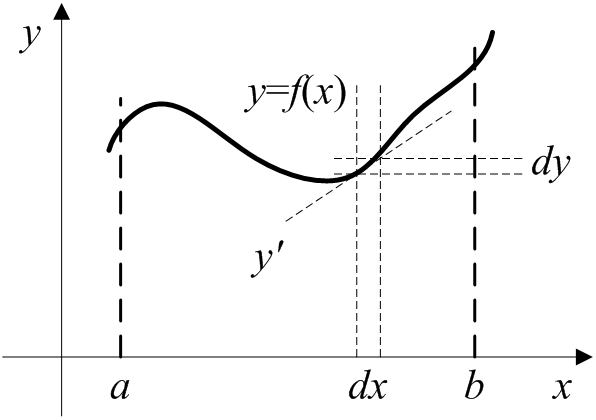
\includegraphics[height=3.5cm]{3.3.png}
\end{figure}

再将这些小区间上的微增量$dy$累积,就能得到$\Delta y$:
\[
\Delta y=\int_a^b{dy}=\int_a^b{y'\cdot dx}
\]
这里,对于每个小区间,$y'$可以认为是$dx$的权重,且$y'$有正有负。
几何上这个权重使得该段对$y$的变化量贡献也有正有负。
最终,$\Delta y$由各个$dy$累积得到。

%============================================================
\subsection{再看定积分的物理意义}

以变速运动为例。
从总体性考察,在一个范围内走过的路程$S\left( t \right) $为过程中的每个小微元$ds\left( t \right)$累积而成:
\[
S\left( t \right) =\int_0^t{ds\left( t \right)}
\]
从局部性考察,极端的时间内走过的路程和时间的比为一个固定的值:
\[
v\left( t \right) =\frac{ds\left( t \right)}{dt}
\]
结合上述两式:
\[
S\left( t \right) =\int_0^t{ds\left( t \right)}=\int_0^t{v\left( t \right) \cdot dt}
\]

\begin{tcolorbox}
“所谓的积分,就是由微分累积而成,所谓的微分,就是积分的局部化分析。”
这就是“教材\cite{book2}”中始终贯穿的微积分的矛盾统一论。
\end{tcolorbox}

%============================================================
\subsection{再看中值定理}

将微分中值定理(拉格朗日定理)和积分中值定义对比看。

用牛顿莱布尼兹公式,拉格朗日定理可以写为:
{\bf 设$F\left( x \right) $在$\left[ a,b \right] $连续,在$\left( a,b \right) $可导,则必有$\xi \in \left( a,b \right) $,使得$f\left( \xi \right) =F'\left( \xi \right) =\frac{F\left( b \right) -F\left( a \right)}{b-a}$。}

对比积分中值定理:
{\bf 若$f\left( x \right) $在$\left[ a,b \right] $上连续,则必有$\xi \in \left( a,b \right) $,使得$\int_a^b{f\left( x \right) dx}=f\left( \xi \right) \left( b-a \right)$。}

可见,两个中值定理描述的是一件事,只不过从两个方面描述而已。
这也反映出微分和积分是对立统一的。




